\section{Experiments}
	\label{sec:experiments}
	\par Two neural networks were tested in this work:
	\begin{enumerate}
		\item \label{itm:snn} \textbf{SNN}: full connected spiking neurons
		\item \label{itm:cnn} \textbf{CNN}: convolutional layer with full connected sigmoid neurons, which were used as a reference.
	\end{enumerate}

	\subsection{Full connected spiking neurons SNN}
	\begin{figure}[H]
		\centering
		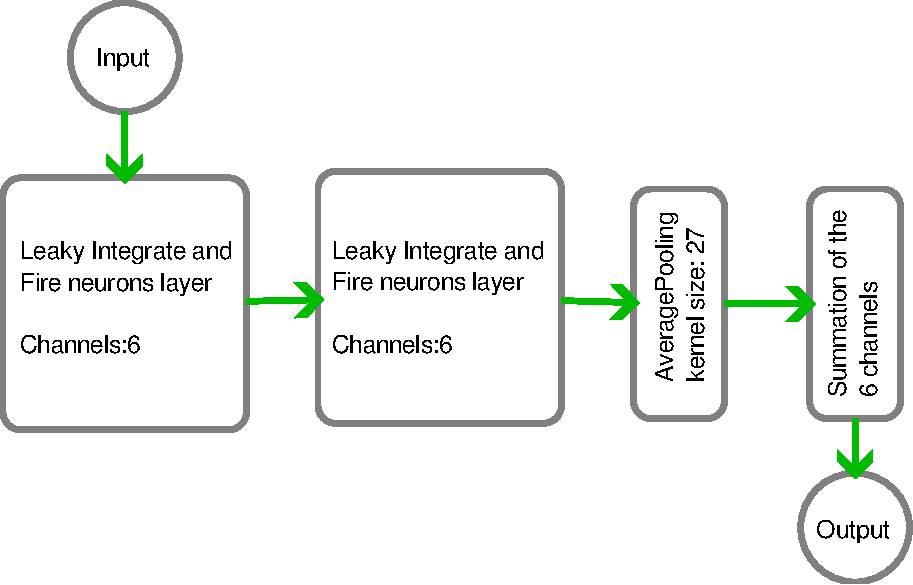
\includegraphics[width=.6\linewidth]{images/architectureSNN}
		\caption{Spiking neural network architecture}
		\label{fig:architecturesnn}
	\end{figure}
	\begin{multicols}{2}
		\par The SNN were trained according to the following parameters:
		\begin{itemize}
			\item \textbf{learning rate}: $2.10^{-4}$
			\item \textbf{test batch size}: 40\%
			\item \textbf{training batch size}: 60\%
			\item \textbf{number of epochs}: 3000
			\item \textbf{loss function}: Cross-entropy
			\item \textbf{optimizer}: Adam ($0.00001 \leq \beta \leq 0.999$)
			\item \textbf{insist}: 4 (amount of times the same data is presented to the network)
			\item \textbf{neuron decay rate}: 0.9 (the rate LIF neuron loses its voltage)
		\end{itemize}
	\columnbreak	
		\begin{lstlisting}[language=Python, caption={SNN architecture}]
self.model = nn.Sequential(
	nn.Linear(inputLength, 4096),
	snn.Leaky(
		beta=neuronDecayRate, 
		spike_grad=spike_grad
	),
	nn.Linear(4096, 27),
	snn.Leaky(
		beta=neuronDecayRate, 
		spike_grad=spike_grad
	),
	nn.AvgPool1d(27, stride=1)
)
\end{lstlisting}
	\end{multicols}


	\subsection{Convolutional layer with full connected sigmoid neurons CNN}

	\begin{figure}[H]
		\centering
		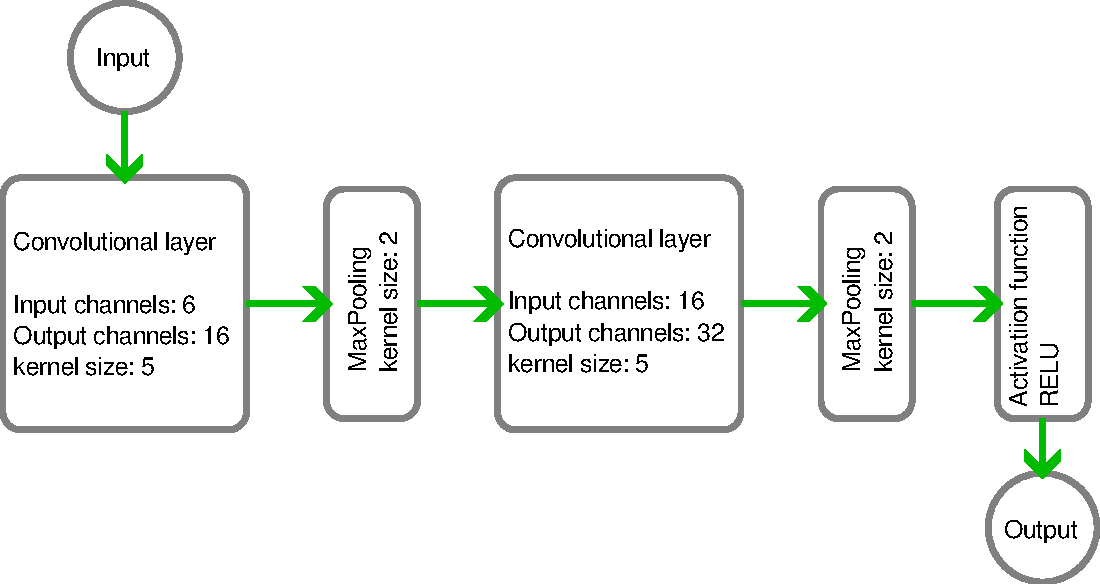
\includegraphics[width=.7\linewidth]{images/architectureCNN}
		\caption{Convolutional neural network architecture}
		\label{fig:architecturecnn}
	\end{figure}

	\begin{multicols}{2}
		\par The CNN were trained according to the following parameters:
		\begin{itemize}
			\item \textbf{learning rate}: $2.10^{-4}$
			\item \textbf{test batch size}: 40\%
			\item \textbf{training batch size}: 60\%
			\item \textbf{number of epochs}: 3000
			\item \textbf{loss function}: Cross-entropy
			\item \textbf{optimizer}: Adam ($0.00001 \leq \beta \leq 0.999$)
		\end{itemize}
	\columnbreak	
		\begin{lstlisting}[language=Python, caption={CNN architecture}]

self.model = nn.Sequential(
	nn.Conv1d(in_channels=6, 
		out_channels=16, kernel_size=5
	),
	nn.MaxPool1d(kernel_size=2),
	
	nn.Conv1d(in_channels=16,
		out_channels=32, kernel_size=5
	),
	nn.MaxPool1d(kernel_size=2),
	
	nn.Flatten(),
	nn.Linear(feature_size, 128),
	nn.ReLU(),
	nn.Linear(128, 27)
)
\end{lstlisting}
	\end{multicols}


	\par The used  database \cite{PRG16} can be found at \href{https://sinc.unl.edu.ar/grants/brain-computer-interfaces/}{https://sinc.unl.edu.ar/grants/brain-computer-interfaces} and consists in a set of EEG data recorded with 6 electrodes during a imagined speech of the words in spanish: 
	"A", "E", "I", "O", "U", "Arriba", "Abajo", "Adelante", "Atrás", "Derecha", "Izquierda".\newline
		
	\par Each channel captured 4096 samples and has the following ids: 'F3','F4', 'C3', 'C4', 'P3', 'P4' according to 10-20 system \cite{ScienceOpenVid:5960cfa8-7fde-441c-8592-35fdb9841499}.
